\documentclass[]{article}

\usepackage[italian]{babel}
\usepackage[margin=20mm, footskip = 20pt]{geometry}
\usepackage{array}
\usepackage{tabularx}
\usepackage{graphicx}
\usepackage{subfiles}
\usepackage{hyperref}
\usepackage{nameref}
\usepackage{titlesec}
\usepackage{longtable}
\usepackage[table]{xcolor}
\usepackage{titling}
\usepackage{lastpage}
\usepackage{ifthen}
\usepackage{calc}
\usepackage{soulutf8}
\usepackage{contour}
\usepackage{float}
\usepackage{fancyhdr}
\usepackage{multirow}
\usepackage{pgfgantt}
\usepackage{lscape}

\newcommand{\hr}{\par\vspace{-.1\ht\strutbox}\noindent\hrulefill\par}

\graphicspath{ {./}
	{./commons/res}
}

%--------------------------------------------------
% Comandi per inserire contenuto del documento
%--------------------------------------------------
\makeatletter

\newcommand\appendToGraphicsPath[1]{%
	\g@addto@macro\Ginput@path{{#1}}%
}

\newcommand{\setTitle}[1]{%
	\newcommand{\@phTitle}{#1}%
}
\newcommand{\phTitle}{\@phTitle}

\newcommand{\setDate}[1]{%
	\newcommand{\@phDate}{#1}%
}
\newcommand{\phDate}{\@phDate}

\newcommand{\setUso}[1]{%
	\newcommand{\@uso}{#1}%
}
\newcommand{\uso}{\@uso}

\newcommand{\setVersione}[1]{%
	\newcommand{\@versione}{#1}%
}
\newcommand{\versione}{\@versione}

\newcommand{\disabilitaVersione}{%
	\renewcommand{\setVersione}[1]{}%
	\renewcommand{\versione}{DISABILITATA}
}

\newcommand{\setResponsabile}[1]{%
	\newcommand{\@responsabile}{#1}%
}
\newcommand{\responsabile}{\@responsabile}

\newcommand{\setRedattori}[1]{%
	\newcommand{\@redattori}{#1}%
}
\newcommand{\redattori}{\@redattori}

\newcommand{\setVerificatori}[1]{%
	\newcommand{\@verificatori}{#1}%
}
\newcommand{\verificatori}{\@verificatori}

\newcommand{\setModifiche}[1]{%
	\newcommand{\@modifiche}{#1}%
}
\newcommand{\modifiche}{\@modifiche}

\makeatother 

%--------------------------------------------------
% Comandi per i documenti esterni e il glossario
%--------------------------------------------------

\newcommand{\dext}[1]{\textsc{#1\textsubscript{\textit{D}}}}

\newcommand{\glock}[1]{\textsc{#1\textsubscript{\textit{G}}}}

%--------------------------------------------------
% Comandi per impostare sottotitoli di quarto e quinto livello
%--------------------------------------------------

\setcounter{secnumdepth}{4}
\setcounter{tocdepth}{4}

\titleformat{\paragraph}
{\normalfont\normalsize\bfseries}{\theparagraph}{1em}{}
\titlespacing*{\paragraph}{0pt}{2.25ex plus 1ex minus .2ex}{1.5ex plus .2ex}

\titleformat{\subparagraph}
{\normalfont\normalsize\bfseries}{\thesubparagraph}{1em}{}
\titlespacing*{\subparagraph}{0pt}{1.75ex plus 1ex minus .2ex}{.75ex plus .1ex}

\appendToGraphicsPath{../../../commons/res/}

%------------------------------
%
% COMANDI DI CONFIGURAZIONE
%
%------------------------------

\setTitle{Verbale riunione \#15}

\setVersione{1.0.0}

\setDate{27-12-2020}

\setResponsabile{Paolo Scanferlato}

\setRedattori{Paolo Scanferlato}

\setVerificatori{Alessandro Dindinelli}

\setUso{Interno}

\setModifiche{
	1.0.0 & Alessandro Dindinelli & Verificatore & 27-12-2020 & Verifica documento\\
	1.0.0 & Paolo Scanferlato & Redattore & 27-12-2020 & Stesura iniziale}

\begin{document}
	
	% Direttive per la creazione del titolo tramite comando maketitle
\title{\huge \textsc{\phTitle{}} \\
	\vspace{11pt} \large \textsc{\phDate{}}}

\author{} % Non toccare
\date{} % Non toccare

%--------------------
% Frontespizio
%--------------------

% Logo del gruppo
\begin{figure}[t!]
	\centering
	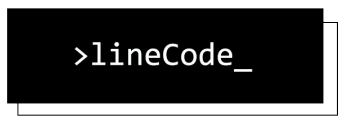
\includegraphics[width=20em]{lclong}
\end{figure}

% Titolo / Nome
\maketitle
\thispagestyle{empty}

% Dati specifici sul doc in forma tabulare
\begin{table}[ht]
	\begin{center}
		\label{tab:Dati sul documento}
		\begin{tabular}{r|l}
			\multicolumn{2}{c}{ \textsc{Dati sul documento} } \\
			\hline
			\textbf{Versione} & \versione{} \\
			\textbf{Uso} & \uso{}  \\
			\textbf{Redattori} & \redattori{} \\
			\textbf{Verificatori} & \verificatori{} \\
			\textbf{Responsabile} & \responsabile{} \\
			\textbf{Destinatari} & lineCode \\
								& prof.\ Vardanega Tullio \\		
								& prof.\ Cardin Riccardo \\
			\ifthenelse{\equal{\uso}{Esterno}}{
								& Sanmarco Informatica
			}{} \\
		\end{tabular}
	\end{center}
\end{table}

\newpage

\renewcommand{\arraystretch}{2} % allarga le righe con dello spazio sotto e sopra
\begin{longtable}[H]{>{\centering\bfseries}m{2cm} >{\centering}m{3.5cm} >{\centering}m{2.5cm} >{\centering}m{3cm} >{\centering\arraybackslash}m{5cm}}
	\rowcolor{lightgray}
	{\textbf{Versione}} & {\textbf{Nominativo}} & {\textbf{Ruolo}} & {\textbf{Data}} & {\textbf{Descrizione}}  \\
	\endfirsthead%
	\rowcolor{lightgray}
	{\textbf{Versione}} & {\textbf{Nominativo}}  & {\textbf{Ruolo}} & {\textbf{Data}} & {\textbf{Descrizione}}  \\
	\endhead%
	\modifiche{}%
\end{longtable}
	
	\newpage
	
	\section{Introduzione}
		\subsection{Luogo e data dell'incontro}
		\begin{itemize}
			\item \textbf{Modalità}: Telematica;
			\item \textbf{Software utilizzato}: Discord;
			\item \textbf{Data}: 23 Dicembre 2020;
			\item \textbf{Ora di inizio}: 16:30;
			\item \textbf{Ora di fine}: 18:30;
		\end{itemize}

		\subsection{Presenze}
		\begin{itemize}
			\item \textbf{Presenti}:
		\begin{itemize}
			\item Matteo Alba
			\item Giacomo Bulbarelli
			\item Alessandro Chimetto
			\item Alessandro Dindinelli
			\item Lucia Fenu
			\item Paolo Scanferlato
			\item Valton Tahiraj
		\end{itemize}
			\item \textbf{Assenti}:
			\begin{itemize}
				\item Nessuno
			\end{itemize}
		\end{itemize}
	
		\subsection{Ordine del giorno}
		\begin{enumerate}
			\item Verifica avanzamento lavori documento \dext{Norme di Progetto};
			\item Suddivisione lavori documento \dext{Piano di Progetto};
			\item Varie ed eventuali.
		\end{enumerate}
	
	\newpage

	\section{Svolgimento}
		\subsection{Verifica avanzamento lavori Norme di Progetto}
		Discussione sulle metriche da inserire nel documento e verifica sullo stato di avanzamento.

		\subsection{Suddivisione lavori Piano di Progetto}
		Il gruppo ha concordato la suddivisione dei lavori per il documento Piano di Progetto.

		\subsection{Discussione sul Glossario}
		Con un rapido scambio di opinioni, si è deciso che il Glossario sarà l'ultimo documento in ordine cronologico ad essere prodotto per la RR.

		\subsection{Modifiche ai verbali}
		Alessandro Chimetto fa presente che nei verbali bisognerebbe identificare univocamente le decisioni prese nelle riunioni per poterle citare nella documentazione. Il gruppo concorda sulla questione e propone le regole per la classificazione. Una tabella le riepilogherà nell'ultima pagina di ogni verbale. \\
		La questione andrà specificata anche nelle \dext{Norme di Progetto}.

		\subsection{Fissata riunione successiva}
		Riunione successiva fissata in:
		\begin{itemize}
			\item \textbf{Data}: 27-12-2020;
			\item \textbf{Ora}: 10:00;
			\item \textbf{Modalità}: Telematica: Discord.
		\end{itemize}
	
	\newpage
	
	\section{Tabella delle decisioni}
	
	\begin{table} [h!]
		\rowcolors{2}{gray!25}{gray!6}
		\begin{center}
			\begin{tabular} { m{2cm} m{14cm} }
				\rowcolor{lightgray}
				\textbf{ID} & \textbf{Decisione} \\
				V15.1 & Suddivisione dei lavori per il documento \dext{Piano di Progetto}:
				\begin{itemize}
					\item Matteo Alba: Pianificazione;
					\item Giacomo Bulbarelli: Analisi dei rischi;
					\item Alessandro Chimetto: Modello di sviluppo - ciclo di vita;
					\item Alessandro Dindinelli: Impostazione e introduzione;
					\item Lucia Fenu: Consuntivo;
					\item Paolo Scanferlato: Preventivo;
					\item Valton Tahiraj: Organigramma.
				\end{itemize} \\
				V15.2 & Glossario sarà l'ultimo documento prodotto in vista della RR.\\
				V15.3 & Verrà aggiunta la tabella delle decisioni prese nelle riunioni nell'ultima pagina di ogni verbale.\\
			\end{tabular}

		\end{center}
	\end{table}
	
\end{document}

